\documentclass[12pt]{article}

\title{Caustics in forward path tracing}
\author{
Shawn Halayka\footnote{sjhalayka@gmail.com}
}


\date{\today\;\currenttime}

\usepackage{datetime}
\usepackage{listings}
\usepackage{cite}
\usepackage{xcolor}
\usepackage{graphicx}
\usepackage{setspace}
\usepackage{amsmath}
\usepackage{url}
\usepackage{amsfonts}
\usepackage{caption}
\usepackage{subcaption}

\usepackage[margin=1in]{geometry}

%\doublespace

\begin{document}

\newcommand{\abs}[1]{\lvert#1\rvert}



\maketitle




\begin{abstract}
In this paper we introduce a method for producting caustics in forward path tracing.
These caustics do not rely on a light location, and as such, do not rely on bidirectional or backward path tracing.
\end{abstract}

\section{Introduction}




\begin{figure} 
\centering
  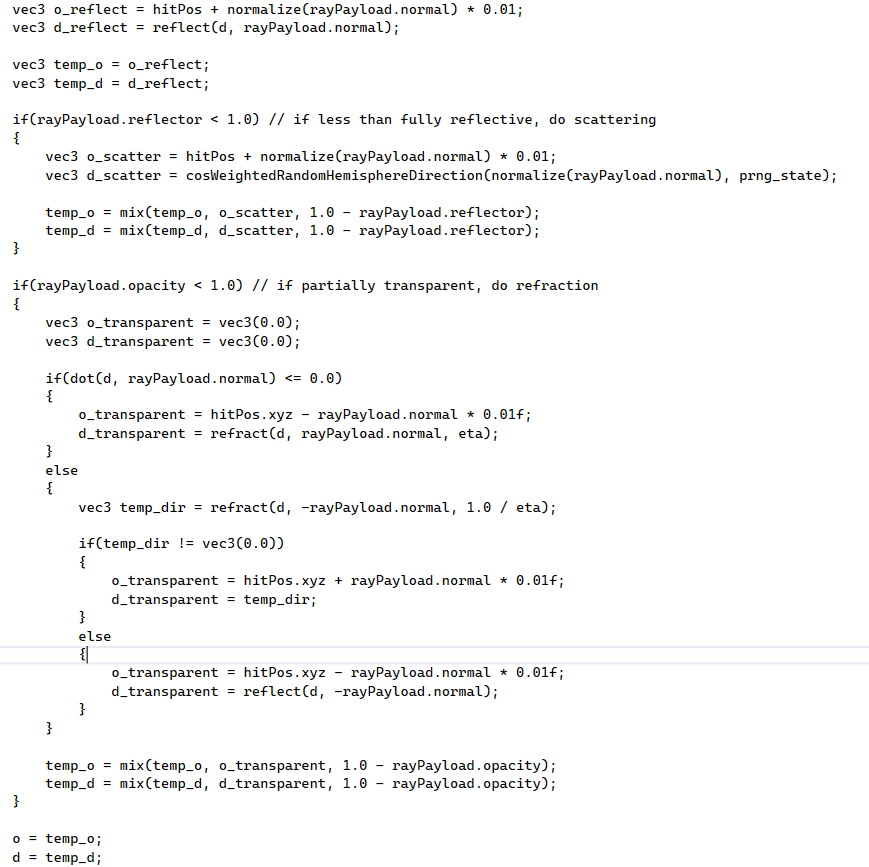
\includegraphics[width = 6 in]{code.png}
  \caption{ Taking into consideration transparent objects.
In essence, instead of always producing a pseudorandom cos-weighted reflection vector, refraction occurs for transparent objects.
}
\end{figure}

\begin{figure} 
\centering
  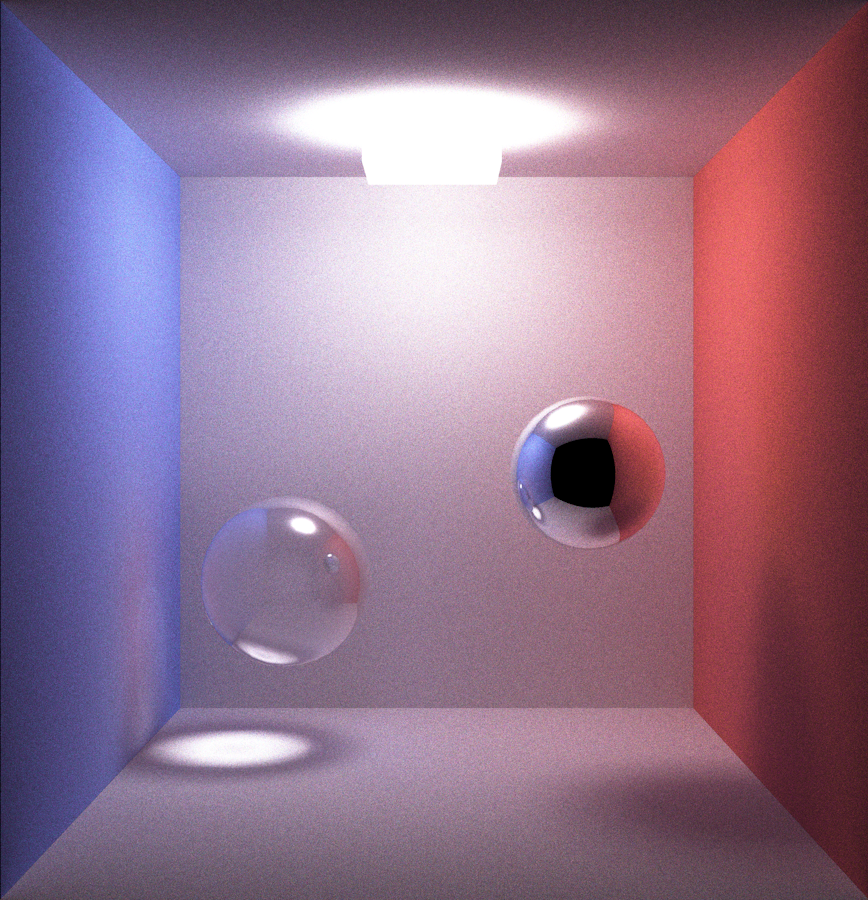
\includegraphics[width = 6 in]{v_rt_reflect_no_chromatic_aberration_low_res.png}
  \caption{ Caption...
}
\end{figure}


\begin{figure} 
\centering
  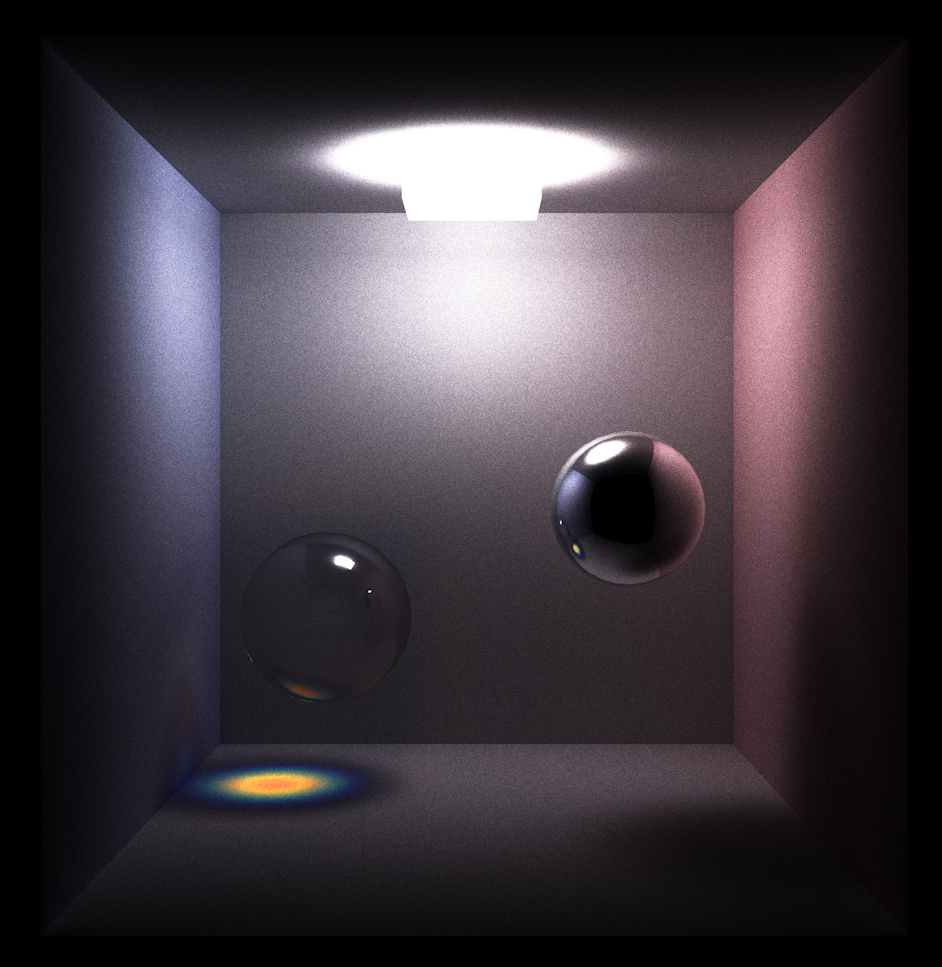
\includegraphics[width = 6 in]{v_rt_reflect_chromatic_aberration_low_res.png}
  \caption{ Caption...
}
\end{figure}

\begin{figure} 
\centering
  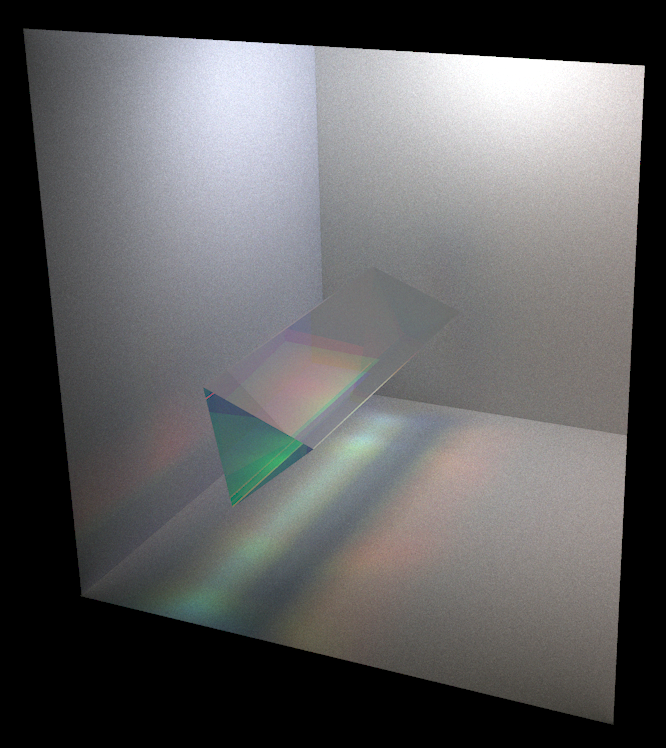
\includegraphics[width = 6 in]{v_rt_reflect_prism.png}
  \caption{ Caption...
}
\end{figure}

\pagebreak

\begin{thebibliography}{9}

\bibitem{fatou} Fatou. Sur les \'equations fonctionnelles. 1919


\end{thebibliography}








\end{document}









